% Homework 8 - CS386
% Russell Miller Winter 2011

\documentclass{article}
\usepackage{anysize}
\usepackage{wasysym}
\usepackage{graphicx}

\marginsize{2cm}{2cm}{2cm}{2cm}

\title{CS386 Homework 8}
\author{Russell Miller\\
Ben Carr}
\date{\today}

\begin{document}

\maketitle

\section{}
\begin{description}
\item[a.]
\ \\
\begin{center}
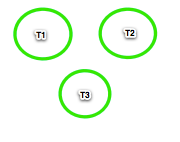
\includegraphics{1a.png}
\end{center}
\emph{There are no precendences in this graph}\\
There are no cycles\\
Therefore it is serializable.
\item[b.]
\ \\
\begin{center}
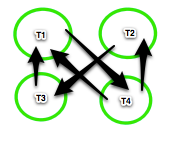
\includegraphics{1b.png}
\end{center}
There is a cycle between T1 and T4. So it is not serializable.
\pagebreak
\item[c.]
\ \\
\begin{center}
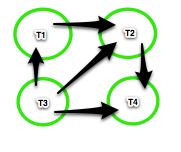
\includegraphics{1c.png}
\end{center}
There are no cycles in all of these edges. So it is serializable.
\item[d.]
\ \\
\begin{center}
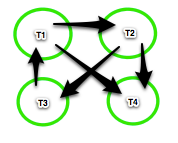
\includegraphics{1d.png}
\end{center}
There is a cycle that goes from T1 to T2 to T3 and back. So it is not serializable.
\end{description}

\section{}
T1 and T2 don't matter because of the checkpoint.\\
\begin{description}
\item[a.]
\ \\
\emph{R1} T3 update A from 4 to 6\\
\emph{R2} T3 update D from 0 to 12\\
\emph{R3} T3 update C from 0 to 9\\
\emph{R4} Commit T3
\item[b.]
\ \\
\emph{U1} T4 update D 2 to 14\\
\emph{U2} Abort T5\\
\emph{U3} T5 update A 6 to 3\\
\emph{U4} T4 update D 12 to 2\\
\emph{U5} T5 update B 9 to 11\\
\emph{U6} T4 update C 10 to 5
\item[c.]
\ \\
A = 6\\
B = 9\\
C = 10\\
D = 12
\end{description}
\section{}


\end{document}
